\documentclass[10pt]{article}

% \setcitestyle{numbers}
\usepackage[numbers]{natbib}
\usepackage[english]{babel}
\usepackage[utf8x]{inputenc}
\usepackage{amsmath}
\usepackage{graphicx}
\usepackage{longtable}
\usepackage[]{hyperref}
\usepackage{comment}
\usepackage{xspace}
\usepackage[usenames]{color}
\usepackage{datetime}
\usepackage{bm}


\title{Measurement of Blended Objects in LSST\\
{\author{
    Jim Bosch\\
    {\em for LSST Data Management}
}}}

\begin{document}

\maketitle

\section{Introduction}

Most LSST objects will overlap one or more of its neighbors enough to affect
naive measurements of their properties.  One of the major challenges in the
deep processing pipeline will be measuring these sources in a way that
corrects for and/or characterizes the effect of these blends.

The measurements of interest can be split up broadly into two categories:
\begin{itemize}
    \item weighted moments (includes aperture fluxes and most centroiders)
    \item forward modeling
\end{itemize}

Most measurements that involve the PSF or a PSF-convolved function as a weight
function can be interpreted in either way, but must be treated as weighted
moments in calculating their uncertainties (i.e. per-pixel variances must
not be used in the weighting) in order to produce unbiased fluxes.

The statistical framework in which weighted moments make sense assumes that
each object is isolated from its neighbors.  As a result, our only option for
these measurements is {\em deblending}, which we define here as any
procedure that attempts to remove neighbors from the pixel values prior to
measurement.

In forward modeling, we convolve a model for the object with our model for
the PSF, compare this model to the data, and either optimize to find
best-fit parameters or explore the full likelihood surface in another way
(e.g. Monte Carlo sampling).  We can use the deblending approach for
forward fitting, simply by fittting each object separately to the deblended
pixels.  However, we can also use {\em simultaneous fitting}, in which we
optimize or sample the models for multiple objects jointly.

Both deblending and simultaneous fitting have some advantages and
disadvantages:
\begin{itemize}
\item Deblending provides no direct way to characterize the uncertainties in
      an object's measurements due to neighbors, while these are naturally
      captured in the full likelihood distribution of a simultaneous fit.
      This likelihood distribution may be very high-dimensional in a fit that
      involves many objects, however, and may be difficult to characterize or
      store.
\item Deblending generally allows for more flexible morphologies than the
      analytic models typically used in forward fitting, which is particularly
      important for nearby galaxies and objects blended with them;
      simultaneous fitting is only statistically well-motivated to the extent
      the models used can reproduce the data.
\item Once deblended pixels are available, fitting objects simultaneously will
      almost always be more computationally expensive than fitting them
      separately to the deblended pixels.  At best, simultaneous fitting will
      have similar performance but still require more complex code.  And
      because we will need to deblend pixels to support some measurement
      algorithms, we'll always have to deblend whether we want to subsequently
      do simultaneous fitting or not.
\end{itemize}

This paper focuses on the problem of blended measurement only; the details of
how we deblend pixels and the models and algorithms we use in simultaneous
fitting will be described elsewhere.

\section{Blend Families and Footprints}

We identify groups of blended objects at the detection stage from their
isophotes at the detection limit; a single simply-connected region of
above-threshold pixels is a {\em parent}, with {\em children} initially
discovered as peaks within that region.  These peaks may not originate in
the same image; we will merge peaks from multiple detection images (e.g.
coadds of different filters or ranges of observation dates).

We call the above-threshold region (and the data structure that defines it) a
\texttt{Footprint}, and the combination of such a region with the values of
the pixels within it (either original data or deblended) a \texttt
{HeavyFootprint}.

For each blend family, in addition to measuring the properties of the children
(either via deblending or simultaneous fitting), we also measure the parent:
we interpret of the region as a single unblended object. This is essentially
an incomplete but useful hedge against overdeblending (we'd like to evaluate
all alternate hypotheses for any combination of peaks belonging to the same
object, but that's infeasible).

\section{Deblended Measurement}

\label{sec:deblender}

The specific approach to deblending we plan to take for LSST is based on
the deblender in the SDSS {\em Photo} pipeline.

Given pixel values $I_{i}$, we create a ``template'' $T_{i,j}$ that represents
an attempt to model the surface brightness of object $j$ at pixel
$i$.\footnote {
    In {\em~Photo}, this template was determined from symmetry arguments and a
    number of heuristics; a full description of how we plan to generate
    templates in LSST is beyond the scope of this paper.
}  We then find the best least-squares linear combination of templates to the
data (ignoring per-pixel variances), solving for coefficients $\alpha_{j}$:
\begin{align}
\bm{\alpha} = \left(\bm{T}^T\bm{T}\right)^{-1}\!\bm{T}^T\bm{I}
\end{align}
Our best-fit prediction for the pixel value vector is thus
$\bm{T}\bm{\alpha}$.
Because this is not the same as the true pixel vector $\bm{I}$, we do not use
the per-object model prediction $\bm{T}\bm{\alpha}$ directly for the deblended
pixel values; instead we reapportion the true per-pixel fluxes according to
the relative predicted contribution from each object:
\begin{align}
D_{i,j} = \frac{
    T_{i,j} \, \alpha_j
}{
    \sum\limits_k T_{i,k} \, \alpha_k
}
I_i
\end{align}

While these deblended pixel values $D_{i,j}$ are what we store in the
\texttt{HeavyFootprint} for each child object, we do not perform measurements
on these values directly for two reasons:
\begin{itemize}
\item $D_{i,j}$ typically has many zero entries, especially for a large blend
    family (i.e. many pixels for which a particular object has no
    contribution).  We include only the nonzero values in the
    \texttt{HeavyFootprint}s for efficiency reasons.
\item Many measurements utilize pixels beyond the blend family's
    \texttt{Footprint}, and in fact may extend to pixels that are in another
    family.
\end{itemize}
To address these issues, we measure deblended objects using the following
procedure:
\begin{enumerate}
\item Replace every above threshold pixel in the image (all
    \texttt{Footprint}s) with randomly generated noise that matches
    the background noise in the image.
\item For each blend family:
    \begin{enumerate}
    \item For each child object in the current blend family:
        \begin{enumerate}
        \item Insert the child's \texttt{HeavyFootprint} into the image,
            replacing (not adding to) any pixels it covers.
        \item Run all measurement algorithms to produce {\em child}
            measurements.
        \item Replace the pixels in the child's \texttt{Footprint} region
            with (the same) random noise again.
        \end{enumerate}
    \item Revert the pixels in the parent \texttt{Footprint} to their original
        values.
    \item Run all measurement algorithms to produce {\em parent} measurements.
    \item Replace the parent \texttt{Footprint} pixels with (the same) random
        noise again.
    \end{enumerate}
\end{enumerate}
This procedure double-counts flux that is not part of a \texttt{Footprint},
but this is considered better than ignoring this flux, because most
measurement algorithms utilize some other procedure for downweighting the
contribution of faraway pixels.

\section{Simultaneous Fitting}

\subsection{Model Selection}

\label{sec:model-selection}

The LSST pipeline will fit both a moving point source and a galaxy model to
each object.  With simultaneous fitting, however, we also have to consider
which models to use for neighbors, and it is clear that allowing for every
possible combination is infeasible (we'd need to fit each blend $2^N$ times,
where $N$ is the number of objects in the blend).

One possible alternative would be to determine the best model for each
object from separate fitting done on deblended pixels, and then fit
simultaneously using just those models.  This makes the simultaneous fitting
essentially useless for classification purposes, however, and it doesn't
reflect the reality that many objects will be impossible to securely classify.

Another option would be to do a single simultaneous fit using a hybrid model
that transitions between a moving point source and a galaxy model.  Because
a non-moving point source is a limit shared by both models, the transition is
continuous, and it should be possible to fit using both sampling methods and
optimization algorithms with some modification (though it will probably be
impossible to use general-purpose algorithms without modification, given the
complexity of the parameter constraints).

\subsection{Minimization}

Simultaneous fitting using optimization algorithms is straightforward from a
mathematical standpoint, but potentially difficult from a computational and
storage standpoint.

Nearly all numerical optimization algorithms involve a matrix factorization
for which the computation complexity is $O(N^2)$ in the number of parameters,
and this makes the worst-case performance scale with the square of the number
of objects in the blend (since the number of total parameters scales linearly
with the number of objects being fit together).  This matrix is typically
sparse for extremely large blends, so sparse matrix methods may avoid this
problem (at an additional cost in overhead).  It is also worth noting that
while the limiting performance for extremely large blends may go as $O(N^2)$,
the bottleneck in fitting galaxies is generally the evaluation of the
models and their first derivatives, which is just $O(N)$ in the number of
parameters.

Optimization-based fitting typically includes an estimate of the parameter
covariance matrix as one of its outputs, and in simultaneous fitting this
covariance matrix naturally includes cross-object terms.  These terms are, of
course, how we characterize how our uncertainty of an object's properties is
affected by its neighbors, and hence are in some sense the reason we're doing
simultaneous fitting at all.  These terms don't fit naturally within the
usual catalog/database model, in which one row corresponds to a single object.
The cross-object terms would need to be stored in some other way, making them
more difficult for users to access.  Perhaps more importantly, for large
blends the total number of outputs is $O(N^2)$ in the number of objects.  The
matrix should be sparse for sufficiently large blends, however, so a storage
scheme that takes advantage of this would address the problem.

If we elect to use hybrid models described in \ref{sec:model-selection}, we
will almost certainly have to develop our own optimization code rather than
adopt an existing third-party code.  High-quality optimization libraries that
can handle complex parameter constraints are extremely rare, and generally
focused on a very specific domain.  It is likely we'd have to develop our own
optimizer even for single-object, non-simultaneous fitting, however, as even
the simpler constraints involved in a single-object galaxy models are
sufficiently complex to give most free optimizers trouble.

\subsection{Monte Carlo Sampling}

One of the advantages of Monte Carlo methods is that they scale better than
optimization methods as dimensionality increases.  If we consider the samples
themselves to be the output of such an algorithm, the storage and catalog
problems we encountered for optimizer outputs simply don't occur: if we sample
simultaneously from a multi-object posterior, we can simply split the storage
and representation of those samples across objects: they'll be the same
samples, but each object's storage will only include its own parameters.
Taken together, the samples represent the joint posterior for all objects in
a blend; taken separately, they represent the marginal posteriors.

The scaling with dimensionality for most Markov Chain Monte Carlo algorithms
depends strongly on the nature of the distribution itself.  The burn-in period
for such algorithms is typically thousands of samples, however, which makes
them impractical for our problem, for which we can only evaluate approximately
200 samples per object (at least when fitting to multi-epoch data).  Instead,
our baseline plan is to use adaptive importance sampling, in which we draw
samples from an analytic distribution that we construct to approximate the
true distribution, then weight those samples according to the true
distribution.  We can then use those weighted samples to modify the analytic
distribution in an iterative sense.  Most importantly, we can do most of these
iterations using a fast approximation to the true likelihood (by fitting to a
coadd instead of multiple epochs, or using a fast but inexact convolution).

Unfortunately, this means we need to construct, draw from, and update
a high-dimensional analytic distribution (typically a mixture Gaussians or
Student's T), and these operations are typically $O(N^2)$ in the total number
of parameters.  As with optimizers, these operations are nearly always
subdominant to the time required to evaluate the likelihood itself.  Instead,
it is the potential complexity of the likelihood surface for large blends that
is most concerning, especially when hybrid models are considered.  In
principle, anything can be done with mixture distributions, but it remains an
open question how efficient this approach will be.

\section{Divide and Conquer for Large Blends}

Regardless of the efficiency of our algorithms in the large-blend limit, it
will be necessary to split the very largest blends and handle them
iteratively.   This will happen automatically, of course, at the boundaries
of our sky pixellization scheme, as some blends will inevitably land on the
boundary between sky patches.  This can be handled straightforwardly by
defining overlapping patches, so that objects near the boundary are processed
twice (once with each patch).  One patch's processing is then selected to
be canonical on an object-by-object basis.  For successful deblending, this
approach essentially relies on individual objects landing entirely within one
patch, along with enough of any neighbors to deblend the primary object.

This requirement will not be met for some large galaxies (or pairs of large
galaxies), and we'll likely have to use a different algorithm for these.  The
same may be true for some extremely large blends that do fit entirely within
one patch, if necessary to keep deblender compute resources minimal.  A multi-
scale approach seems natural here - start on a binned image of a larger sky
area, and use this to generate templates for the largest objects.  We then
move to subimages at high resolution resolution to produce templates for
smaller object, until we return to the regular pixel scale. The final linear
fit for template coeffients ($\bm{\alpha}$) could then be done on a
combination of regular pixels and binned superpixels, depending on which
templates are active in a particular region, and may make use of sparse matrix
methods.  This approach may need to be iterative.

We may or may not want to use the same divisions for simultaneous fitting.  By
the time we reach the simultaneous fitting stage, we'll have some idea of the
extents of children, and we may be able to find a divisions that require
smaller overlap regions and/or a smaller number of objects with duplicate
processing (by drawing boundaries that only touch a small number of compact
objects). Patch boundaries will also be less important, as we'll be able to
iterate directly over blend families (and hence only worry about sky patches
for I/O).  It may even be unnecessary to do any kind of divide-and-conquer for
simultaneous fitting if we use sparse matrix methods and parallelize in a way
that splits likelihood evaluation over multiple cores.

\section{Iterative Deblending and Fitting}

Thus far we've considered simultaneous fitting as an optional stage following
per-pixel deblending.  We can also use the results of a simultaneous fit as
the weighted templates ($\bm{T}\bm{\alpha}$) in a subsequent deblending step.

We've already highlighted model flexibility as an advantage of deblended
measurement over simultaneous fitting, and this approach would remove
some of that advantage, because the models used in simultaneous fitting are
not as flexible as {\em e.g.} SDSS-style templates derived from symmetry
arguments.  It wouldn't remove the advantage entirely, because we apportion
the original pixel values according to the relative template contributions
rather than using the template values directly.

Even so, using simultaneous models as deblend templates does present some
advantages over more flexible templates:
\begin{itemize}
\item We don't currently know how we're going to translate templates from
coadds (where they're derived, at least for deep processing) to individual
epochs, which involves both a change in PSF and coordinate system, and
analytic models are one candidate.
\item Using models provides a natural way to include prior information and
constraints on the deblending, such as a requirement that deblending produce
physically reasonable colors.
\item It may be possible to propagate cross-object uncertainty estimates
from a simultaneous fit into the deblend and hence moments-based
measurements.  A straightforward (but expensive) approach would be to repeat
the suite of moments-based measurements on deblended pixels derived from model
parameters at each sample point in a Monte Carlo simultaneous fit.
\end{itemize}

\section{LSST Pipeline Straw-Man Proposal}

The above sections describe a number of algorithmic options that can be
combined in myriad ways.  In this section, we describe (at summary level) a
full baseline pipeline and a few top-priority alternatives. The baseline plan
is outlined in Figure~\ref{fig:flowchart}, with details described below.

The first major processing stage described here is the Deblender [P1], which
we imagine as an algorithm very similar to that the SDSS {\em Photo} deblender
described in Section~\ref{sec:deblender}, likely using a symmetry ansatz to
define templates.  The inputs will be a detection catalog containing merged
{\texttt Footprints} and {\texttt Peaks} from all detection images [D1], and
at least one coadd image per filter [D2].  We may have multiple input coadds
for each filter, representing different depth vs. resolution tradeoffs or
different epochs, as well as some coadds that represent combinations of data
from different filters. The details of these inputs and the parallelization
and data flow within the deblender itself are beyond the scope of this
document. The deblender outputs will include the deblend templates [D7] for
each filter and deblended pixel values for both direct [D5] and PSF-matched
[D6] coadds (generated by sequentially replacing neighbors with noise, as
described in Section~{sec:deblender}).

\begin{figure}
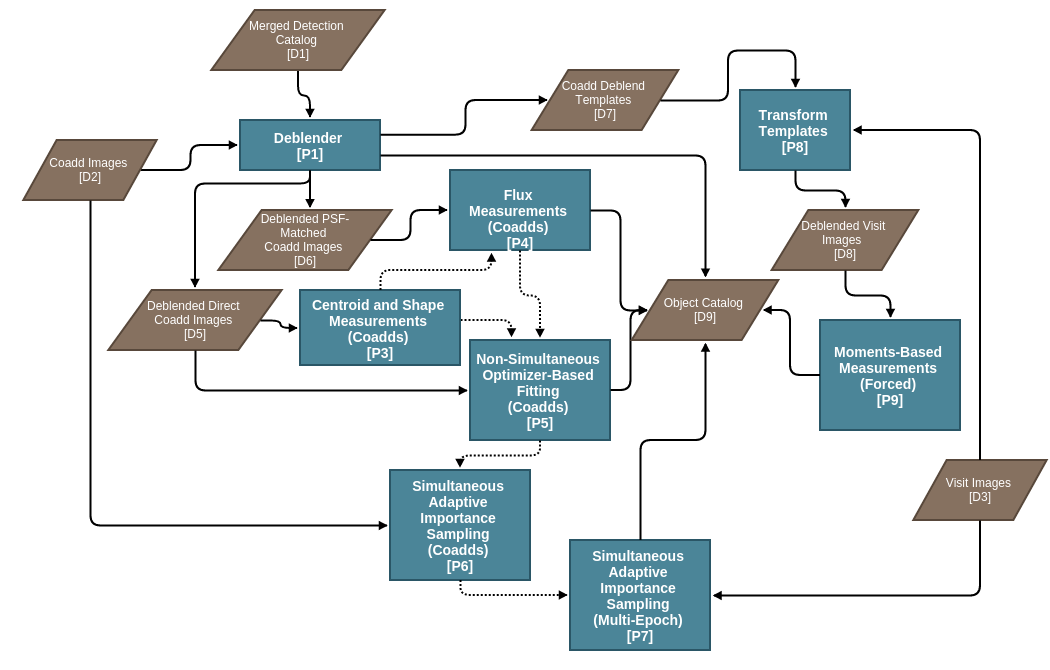
\includegraphics[width=\columnwidth]{flowchart.png}
\caption{Pipeline for Blended Measurement}
\label{fig:flowchart}
\end{figure}

\end{document}